\section{Results}

\subsection{Data usage across operating systems and scenarios}

Total network data usage across all operating systems and applicable scenarios is presented in Figure~\ref{fig-all-tasks-chart}. To keep the results comparable and avoid dominance by bulk transfers, we excluded traffic to domains used for application and system update payload delivery (large binary downloads). However, this exclusion was not perfect, and some residual update-related traffic remains in the dataset. Generally, we expect lower network traffic in configurations with fewer Google services present.

\begin{figure}
	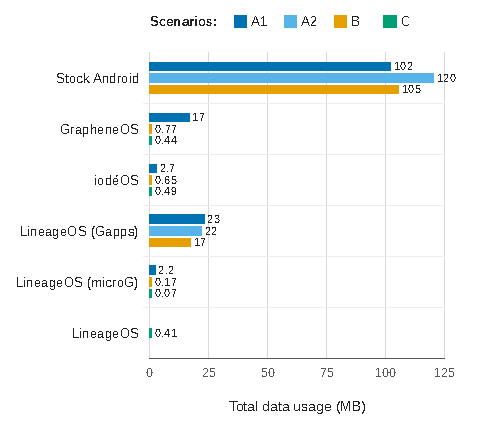
\includegraphics[width=\columnwidth]{images/all-tasks-data-usage-acm.pdf}
	\caption{Total data usage aggregated across all measurement tasks. Scenario applicability varies by system.} \label{fig-all-tasks-chart}
\end{figure}

For initial device setup, stock Android shows the highest data usage (71-85 MB). The modest reductions between privacy-adjusted scenarios indicate that configuration choices provide little control over automatic updates and background activity. Configurations incorporating more Google services generate higher traffic, while de-Googled baselines demonstrate substantially reduced data exchange. LineageOS with official Google Play Services generates substantially less traffic (16-21 MB) than stock Android due to its minimal base system. However, it remains considerably higher than configurations without proprietary Google services, with the microG variant and the Google-free installation achieving notable further reductions (0-3 MB). For GrapheneOS, Scenario B demonstrates that even when sandboxed Google Play Services are installed and granted network and background permissions, they remain largely inactive when not deliberately invoked. This contrasts with the persistent background activity characteristic of integrated GMS deployments.

Network activity observed during system idle following a reboot shows stock Android again with the highest data usage, though Scenario B exhibits unexpectedly elevated traffic compared to both Scenario A2 and Scenario A1. This anomaly results from substantial background communication with \textit{www.gstatic.com}, likely triggered by automatic updates or other background activity during the measurement period.

LineageOS in Scenario C similarly deviates from anticipated patterns, generating more idle traffic than its microG variant. GrapheneOS exhibits nearly identical traffic in Scenarios B and C, confirming that sandboxed Google Play Services generate minimal background activity when not actively in use.

During basic application interactions that should not require Internet connectivity, stock Android dominates with substantial data usage caused mostly by uncontrolled updates. All alternative distributions demonstrate significantly lower traffic, with de-Googled configurations remaining effectively silent. Notably, whenever official Google Play Services were present and a Google account was logged in, at least one request to Google infrastructure occurred.

\subsection{Domain distribution and Google dependencies}

\begin{figure}
	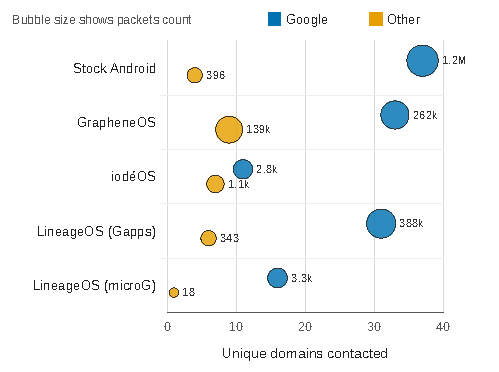
\includegraphics[width=\columnwidth]{images/os-domains-packets-acm.pdf}
	\caption{Domains contacted in Scenario A1 aggregated for all tasks, grouped by operating system and by Google-related and other endpoints. Bubble size represents the total number of packets exchanged with each group.} \label{fig-domains-chart}
\end{figure}

Figure \ref{fig-domains-chart} presents the domain-level distribution of network traffic for Scenarios A1 and B. These scenarios were selected as the most realistic configurations, incorporating essential Google functionality while differing in account linkage and privacy-related settings. Overall traffic is dominated by large content transfers, as systems download necessary resources and updates. Stock Android contacts the widest range of Google domains, distributing traffic across numerous endpoints. Alternative systems show reduced Google communication, although patterns vary by design. GrapheneOS generates more requests than microG-based systems, as it downloads Google services on demand from its own application store. iod\'eOS and LineageOS with microG contact fewer Google servers overall, as microG minimizes connectivity while still enabling basic functionality. iod\'eOS also relies on some Mozilla infrastructure not present in other systems.

Table \ref{tab:domains-mechanisms} shows the infrastructure dependencies for core system functions. LineageOS variants remain closest to stock Android, relying entirely on Google servers for connectivity checks, remote provisioning, and location assistance. iod\'eOS adopts an intermediate position, using independent infrastructure for connectivity checks while still depending on Google for remote provisioning and location services. GrapheneOS demonstrates the strongest de-Googling, substituting all three functions with its own or independently operated infrastructure. Both iod\'eOS and GrapheneOS expose these mechanisms through explicit system settings toggles, though GrapheneOS offers more granular control: users may choose between its independent proxy infrastructure and official Google servers for each function, with the default configured to avoid Google connections entirely.

\begin{table*}
	\caption{Domains observed for connectivity check, remote provisioning, and location assistance.}
	\label{tab:domains-mechanisms}
	\begin{tabular}{llll}
		\toprule
		System & Connectivity check & Remote provisioning & Location assistance \\
		\midrule
		Stock Android & connectivitycheck.gstatic.com & -- & supl.google.com, agnss.goog \\
		LineageOS & connectivitycheck.gstatic.com & remoteprovisioning.googleapis.com & supl.google.com, agnss.goog \\
		iod\'eOS & captiveportal.kuketz.de & remoteprovisioning.googleapis.com & supl.google.com \\
		GrapheneOS & connectivitycheck.grapheneos.network & remoteprovisioning.grapheneos.org & gs-loc.apple.grapheneos.org \\
		\bottomrule
	\end{tabular}
\end{table*}

\subsection{Additional findings}

Beyond aggregate traffic measurements, we examined specific data transmissions revealed through TLS interception and payload analysis. A subset of these observations originates from earlier experiments performed on Android 14. They could not be reconfirmed on Android 16, as the Frida-based method we employed became unsuccessful, though we expect the general patterns to persist. GrapheneOS blocked all our instrumentation attempts, so we cannot verify what data these requests contained. However, the substantially lower request volume suggests that sandboxed Google Play Services likely transmit less complete or less authentic information.

Android's check-in mechanism transmits device identifiers to Google infrastructure. On stock systems, this includes the real IMEI and hardware serial number. In contrast, microG employs a privacy-preserving approach by generating randomized, rotating identifiers including fake IMEIs (consistently prefixed with \texttt{35503104}), MAC addresses (with OUI \texttt{b4:07:f9}), and a synthetic serial number displayed in microG settings. The Android ID field in microG requests is frequently empty or zeroed. However, microG still transmits authentic device characteristics including model, Android version, and time zone, enabling functional compatibility while obscuring persistent hardware identifiers.

We observed requests to \textit{app-measurement.com} on systems with Google services present, primarily on stock Android. These transmissions contained application package names, installation sources (Google Play, Aurora Store, manual), versions, and the system theme preference. Information about installed applications was transmitted even for those that were never launched.

The Google Advertising ID (ADID) was observed in multiple requests on stock Android, formatted as a UUID. This value remained constant across different requests, confirming its persistence as a cross-application tracking mechanism. After a manual reset in system settings, the ADID was transmitted as all zeros, indicating the identifier was actually cleared rather than immediately regenerated.

When enabled, microG performs network geolocation without Google infrastructure by querying a selected provider, in our case \textit{api.position.xyz}. The request transmits data about nearby cell towers and returns approximate coordinates. Location fixes were obtained almost immediately after enabling this feature, compared to significantly slower location acquisition prior to activation.

We compared Google Play Store with Aurora Store, a popular application source in alternative Android distributions, by downloading the same application from each platform. Both stores retrieved identical packages from the same Google CDN infrastructure. However, the Play Store generated 106 requests, while Aurora Store produced 93, omitting Google telemetry connections, but adding lookups to Exodus Privacy and Plexus databases for tracker analysis and compatibility ratings. Aurora achieves functional equivalence by mimicking Play Store user agents and headers, using shared anonymous credentials rather than a personal account.

\subsection{Google Takeout}

We submitted Google Takeout requests for accounts we used, and analyzed the Android device data. Four distinct Google service configurations were examined: stock Android as a baseline, LineageOS with Gapps as an alternative system incorporating Google services, LineageOS with microG as an open-source reimplementation (iod\'eOS includes an identical microG version), and GrapheneOS as a representative of a sandboxed approach. For every logged-in system, a corresponding entry appeared in \texttt{devices.json}, including device model, OS version, country, language, registration timestamp, and last activity time. However, the depth of telemetry varied considerably across configurations, as summarized in Table \ref{tab:takeout-comparison}.

Both systems using official Google services reported a large list of installed applications. GrapheneOS reported only four preinstalled applications, two of which were GrapheneOS-specific. In contrast, microG did not create any application-related entry. Additionally, stock Android and LineageOS with GMS both transmitted authentic hardware identifiers including IMEI and serial number. GrapheneOS submitted a falsified serial number and omitted IMEI entirely. Again, microG did not create an additional device-related entry, so these identifiers were not present. A Pixel-specific telemetry directory, present only for stock Android and LineageOS with GMS, contained extensive hardware monitoring data including power measurements, Wi-Fi signal logs, battery capacity readings, thermal samples, and battery cycle entries. LineageOS reported less granular telemetry than stock Android, indicating that while basic Pixel telemetry infrastructure remains functional, the depth of hardware monitoring is reduced compared to the proprietary stock implementation.

\begin{table}
	\caption{Comparison of Google Takeout data across Android configurations.}
	\label{tab:takeout-comparison}
	\begin{tabular}{llll}
		\toprule
		System & Device IDs & Apps & Pixel telem. \\
		\midrule
		Stock Android & IMEI, serial & Extensive & Full \\
		Lineage (Gapps) & IMEI, serial & Extensive & Reduced \\
		Lineage (microG) & -- & -- & -- \\
		GrapheneOS & Falsified serial & 4 apps & -- \\
		\bottomrule
	\end{tabular}
\end{table}